\documentclass[a4paper]{article}

\usepackage[english]{babel}
\usepackage[utf8]{inputenc}
\usepackage{amsmath}
\usepackage{graphicx}
\usepackage[colorinlistoftodos]{todonotes}

\title{Electric Circuits 307 - Operational Amplifiers}

\author{Josh Lofy}

\date{\today}

\begin{document}
\maketitle

\begin{abstract}
In this lab we used a 741 style operational amplifier to create a series of different circuits.  These circuits used both inverting and non-inverting amplifiers.  I will also discuss the output signals created by these circuits, and how they can be used in real world cases.
\end{abstract}

\section{Introduction}

Amplifiers are helpful tools that we can use to manipulate signals.  These manipulations are the same as performing mathematical logic rules to the signal.  

In this lab we created an inverting amplifier, a non-inverting amplifier, a follower circuit, and a summing amplifier.  However, our summing aplifier did not actually sum an incoming signal.  Instead, we offset our output signal of a non-inverting amplifier by -3V and then used a second amplifier to uninvert the signal.  This produced the signal we were looking for, but did not actually create a singal summing amplifier that created a +3v voltage offset.

\section{Circuit Design}

\subsection{Circuit Requirements}

\begin{itemize}
\item Frequency generator
\item Oscilloscope
\item LM741CN Amplifier
\item Breadboard
\item Wires
\item 1k Ohm Resistor
\item 10k Ohm Resistor
\item Resistor Decade Box
\end{itemize}

\subsection{Inverting Amplifier}

For our inverting amplifier we created a circuit with a gain of A=-100.  In this case, the negative represents that the signal is inverted.  The value shows that the signal will be amplified one hundred times.  To do this, we use a resistor that is 100 times larger than our incoming resistor for our feedback signal.  Figure 1 shows the circuit design.

\begin{figure}
\centering
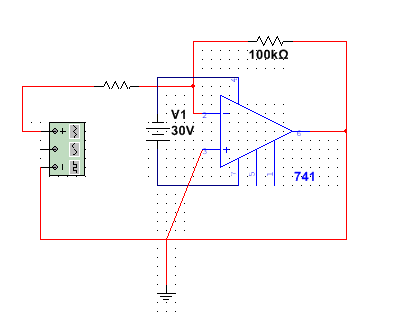
\includegraphics[width=0.65\textwidth]{Inverting100.png}
\caption{\label{fig:Inverting}Shows an inverting amplifier circuit.  With a 1k resistor on the input this circuit will create a A=-100 amplifier.}
\end{figure}

\subsection{Non-Inverting Amplifier}

For our non-inverting amplifier, we create an output signal that is the same phase as the input signal.  Their transfer function for the gain is also quite different.  The gain is instead calculated by the gain function \[A=1+R2/R1\]

Where R2 is the resistor between the inverting input and the ground, and R1 is on the output of the amplifier to the node with R2 and the inverting input.  Using this set up we were able to create a circuit that amplified our signal to 1.1 times the original signal.  

\subsection{Follower}

Our follower amplifier was a simple circuit that stabilized our initial signal.  It's primary real purpose is to act as a current gain between 2 circuits of different impedence.  However, it's voltage signal, the signal we are interested in in most other circuits, is virtually unchanged.  This gives us an effective voltage gain of 1.  It's circuit design is shown in Figure 2.

\begin{figure}
\centering
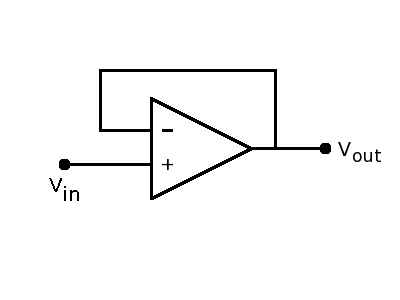
\includegraphics[width=0.4\textwidth]{Follow.png}
\caption{\label{fig:follower}A simple representation of a Follower Amplifier.}
\end{figure}

\section{Discussion}

In our lab, we were supposed to create a summing circuit using just the amplifier that would create a signal that was offset by, \[V=+3 Volts\]

However, what we really created were a circuit that amplified our signal, inverted it, and then offset the output by -3 volts.  We then used an inverting amplifier to right our signal back again.

In retrospect, it would have been better to follow the design from our midterm that used Kirchoff's Circuit Laws to create a proper amplifer with the correct output signal for the correct input signal.  What we created was a signal that looked like the output that we wanted, but had little resemblance to the actual circuit we wanted and was much more complicated.

\section{Conclusion}

We were able to produce accurately the proper output signal for each circuit.  However, as discussed in the discussion section, we did not necessarily created all fo the amplifier circuits as we had thought.  Because of this, I think it would be important to review and learn from this lab for future study into our circuits.  

For me, this was a learning experience in remembering the roots of the electric circuits, rather than continuing to focus on learning ever newer and more powerful transfer functions.  Remembering the basics of Kirchoff's Circuit Laws would have saved me both time in the design and implification of the circuit, and some points on my midterm.

\end{document}